\documentclass[a4paper,11pt]{article}

\usepackage[czech]{babel}
\usepackage[utf8]{inputenc}
\usepackage{graphics}
\usepackage{caption}
\usepackage[hidelinks]{hyperref}
%velikost stránky
\usepackage[left=1.5cm,text={18cm, 25cm},top=2.5cm]{geometry}


%%%%%%%%%%%%%%%%%%%%%%%%%%%%%%%%%%%%%%%%%%%%%%%%%%%%%%%%%%%%%%%%%%%%%%%%%%%%%
\begin{document}
\begin{center}
\Huge
\textsc{\LARGE Vysoké učení technické v Brně\\[-4.5mm] Fakulta informačních technologií}\\
\vspace{\stretch{0.100}}

\includegraphics{logo_fit.png}\\
\vspace{\stretch{0.100}}
{\LARGE Modelování a simulace\\[0mm]2014/2015}\\[2mm]
Plynová krize v Evropě\\
\vspace{\stretch{0.618}}
\end{center}
{\Large 
Marek Fiala, xfiala46\\
Martin Janoušek, xjanou14
\hfill
\today 
}

\thispagestyle{empty}
\newpage

\thispagestyle{empty}
\tableofcontents
\newpage


\section{Úvod} 

%Úvod musí vysvětlit, proč se celá práce dělá a proč má uživatel výsledků váš dokument číst (prosím, projekt sice děláte pro získání zápočtu v IMS, ale mohou existovat i jiné důvody). Případně, co se při čtení dozví.

%Například: 
%v této práci je řešena implementace ..., která bude použita pro sestavení modelu ...
%na základě modelu a simulačních experimentů bude ukázáno chování systému ... v podmínkách ...
%smyslem experimentů je demonstrovat, že pokud by ..., pak by ...
%Poznámka: u vyžádaných zpráv se může uvést, že zpráva vznikla na základě požadavku ... (u školní práce takto zdůvod'novat projekt ovšem nelze, že). Je velmi praktické zdůvodnit, v čem je práce náročná a proto přínos autora nepopiratelný (např. pro zpracování modelu bylo nutno nastudovat ..., zpracovat, ... model je ve svém oboru zajímavý/ojedinělý v ...).


Tato práce popisuje řešení implementace diskrétního modelu produkce, spotřeby a přepravy plynu v zemích Česká republika, Polsko, Slovensko, Maďarsko a Ukrajina.

Na základě vytvořeného modelu a simulačních experimentů bude ukázána závislost jednotlivých zemí na dovozu zemního plynu z Ruska, 
užitečnost možného dovážení zkapalněného zemního plynu \textit{(LNG)} z USA a míra připravenosti výše zmiňovaných zemí na možnou plynou krizi.

Smyslem experimentů je demonstrovat odolnost daných států vůči embargu na zemní plyn ze strany Ruska a jejich schopnost udržet normální běh státu v tomto stavu.
Dalším smyslem je hledání nového zdroje zemního plynu, kterým by se zmírnila závislost
na zemním plynu dováženém z Ruska.


\subsection{Autoři a hlavní zdroje informací}
\subsubsection{Autoři}
%Podkapitoly:
%kapitola 1.1: Kdo se na práci podílel jako autor, odborný konzultant, dodavatel odborných faktů, význačné zdroje literatury/fakt, ...
%je ideální, pokud jste vaši koncepci konzultovali s nějakou autoritou v oboru (v IMS projektu to je hodnoceno, ovšem není vyžadováno)
%pokud nebudete mít odborného konzultanta, nevadí. Nelze ovšem tvrdit, že jste celé dílo vymysleli s nulovou interakcí s okolím a literaturou.


\begin{itemize}
\item Marek Fiala, xfiala46@stud.fit.vutbr.cz
\item Martin Janoušek, xjanou14@stud.fit.vutbr.cz
\end{itemize}

\subsubsection{Hlavní zdroje informací}
Za hlavní zdroj informací byl použit elektronický sborník Natural Gas Information \cite{IEA}\footnote{konkrétně ten vydaný v roce 2014},
který je každoročně vydáván \textit{Mezinárodní energetickou agenturou}\footnote{viz. \url{www.iea.org}}.
Tento elektronický sborník se zabívá požadavky a zásobami plynu v zemích po celém světě.


Dalším důležitým zdrojem informací byla webová stránka asociace \textit{Gas Infrastructure Europe (GIE)}\footnote{viz. \url{www.gie.eu.com}}.

\subsection{Validace modelu}

%kapitola 1.2: V jakém prostředí a za jakých podmínek probíhalo experimentální ověřování validity modelu – pokud čtenář/zadavatel vaší zprávy neuvěří ve validitu vašeho modelu, obvykle vaši práci odmítne už v tomto okamžiku.

Ověřování modelu probíhalo experimentování s modelem a to v rámci různých testů.
Výsledky těchto testů byly srovnávány s dostupnými informacemi a také s výsledky,
které byly dosaženy analitickými metodami.
Jako kontrolní informace byla využita studie na téma \textit{Embargo ruského plynu}\footnote{Dostupné na \url{www.regjeringen.no/upload/OED/pdf\%20filer/Brussel/Hoeffler_Gas_Embargo.pdf}}.
Výsledky testů byly také srovnávány napříč mezi sebou, což neověřilo správnost celého modelu, ale shodnosti jednotlivých komponent.

\subsection{Zadání projektu}

Oficiální zadání projektu je k dispozici na stránkách \url{http://perchta.fit.vutbr.cz:8000/vyuka-ims/34}.

\begin{quotation}
\uv{Navrhněte diskrétní model produkce, spotřeby a přepravy plynu v zemích okolo České republiky
(Polsko, ČR, Slovensko, Maďarsko, Ukrajina).
Za místa produkce považujte místa aktuálních (a uvažovaných) přístavních terminálů na LNG v Evropě,
podzemní zásobníky v daných zemí (včetně jejich kapacity) a Rusko.
Každou zemi považujte v modelu za jeden uzel produkce a spotřeby (neuvažují se místní rozvody plynu).
Modelujte současnou přepravní síť mezi uzly.
Síť dle potřeb rozšiřte o další uzly a země. Navrhněte a zdůvodněte přepravní doby mezi uzly v jednotce množství za hodinu
(př. uzel Rusko produkuje do přepravního kanálu na Ukrajinu X množství každou hodinu.
Přepravní doba z uzlu Rusko do uzlu Ukrajina je Y hodin.).
Zkoumejte dostupnost plynu v uzlech v různých obdobích roku (zimní spotřeba, letní spotřeba)
v různých scénářích (zprovoznění terminálu LNG pro dovoz z USA,
Ukrajina přeruší transportní cestu, Rusko přestane dodávat apod.).}
\end{quotation}

\subsection{Zkoumané scénáře}

\begin{enumerate}
\item[I.] \textbf{Současná situace}

Zkoumání současného stavu včetně dodávek z Ruska.
Scénář je vhodný z důvodu následného ověřování modelu.

\item[II.] \textbf{Zastavení dodávek z Ruska}

Zjištění doby, která uplyne od zastavení dodávek z Ruska do vyčerpání zásob u jednotlivých zemí.

\item[III.] \textbf{Dodávání plynu z USA po celý rok}

Simulace stavu, kdy se začne dovážet plyn z USA a Rusko omezí dodávky plynu.

\item[IV.] \textbf{Dovoz plynu z USA pouze v letním období}

Varianta předchozího scénáře s dodávkami plynu z USA pouze v letním období.

\item[V.] \textbf{Dosatečné zásoby na jeden rok}

Zjišťování dostatečné kapacity zásobníků plynu v jednotlivých zemích
tak, aby v případě plynové krize vystačily po dobu jednoho roku.
\end{enumerate}

\newpage

\section{Rozbor tématu a použitých metod/technologií}

%Shrnutí všech podstatných faktů, které se týkají zkoumaného systému (co možná nejvěcnějším a technickým (ideálně formálně matematickým) přístupem, žádné literární příběhy). Podstatná fakta o systému musí být zdůvodněna a podepřena důvěryhodným zdrojem (vědecký článek, kniha, osobní měření a zjišťování). Pokud budete tvrdit, že ovce na pastvě sežere dvě kila trávy za den, musí existovat jiný (důvěryhodný) zdroj, který to potvrdí. Toto shrnutí určuje míru důvěryhodnosti vašeho modelu (nikdo nechce výsledky z nedůvěryhodného modelu). Pokud nebudou uvedeny zdroje faktů o vašem systému, hrozí ztráta bodů.



\subsection{Popis použitých metod a technologii}

%kapitola 2.1: Popis použitých postupů pro vytvoření modelu a zdůvodnění, proč jsou pro zadaný problém vhodné. Zdůvodnění může být podpořeno ukázáním alternativního přístupu a srovnáním s tím vaším. Čtenář musí mít jistotu, že zvolené nástroje/postupy/technologie jsou ideální pro řešení zadaného problému (ovšem, "dělám to v Javě, protože momentálně Java frčí..." nemusí zadavatele studie uspokojit).

Pro implementaci byl zvolen jazyk C++ a to ve variantě bez knihoven podporujících simulaci.
Důvodem tohoto rozhodnutí byla rychlost spustitelného programu a také to,
že veškeré události v modelu se vykonávají diskrétně v intervalech po jedné hodině.
Modelového času \cite[str,21]{IMS} pro účeli tohoto modelu lze tedy docílit
jednoduše vykonáním všech
událostí se stejným počátečním časem v jedné iteraci cyklu.

\subsection{Popis původu použitých metod/technologií}
%kapitola 2.2: Popis původu použitých metod/technologií (odkud byly získány (odkazy), zda-li jsou vytvořeny autorem) - převzaté části dokumentovat (specificky, pokud k nim přísluší nějaké autorské oprávnění/licence). Zdůvodnit potřebu vytvoření vlastních metod/nástrojů/algoritmů. Ve většině případů budete přebírat již navržené metody/algoritmy/definice/nástroje a je to pro školní projekt typické. Stejně tak je typické, že studenti chybně vymýšlí již hotové věci a dojdou k naprostému nesmyslu - je třeba toto nebezpečí eleminovat v tomto zdůvodnění.

%Velmi důležité, až fanaticky povinné, kontrolované a hodnocené: na každém místě v textu, kde se poprvé objeví pojem z předmětu IMS bude v závorce uveden odkaz na předmět a číslo slajdu, na kterém je pojem definován. Pokud bude významný pojem z předmětu IMS takto nedokumentován v textu a zjevně bude používán nevhodným nebo nepřesným způsobem, bude tento fakt hodnocen bodovou ztrátou. Tento požadavek je míněn s naprostou vážností. Cílem je vyhnout se studentské tvůrčí činnosti ve vysvětlování známých pojmů, což mnohdy vede k naprostým bludům, ztrátě bodů a zápočtů. Pokud student pojem cituje korektně a přesto nekorektně používá, bude to hodnoceno dvojnásobnou bodovou ztrátou.

Pro získání přenosové doby plynu mezi jednotlivými zeměmi a přístavními terminály,
bylo nutné vypočítat tyto hodnotu z délky jednotlivých plynovodů a rychlosti plynu,
který v nich proudí.
Stejně tak množství plynu, se kterým se pracuje za dobu jedné hodiny,
bylo nutné vypočítat z hodnot, které jsou udány v množství za hodinu.
Všechny vzorce a zdroje jsou uvedeny v kapitole \ref{Rozbor}. 

\subsection{Rozbor tématu}\label{Rozbor}

Zemní plyn je přírodní hořlavý plyn využívaný jako významné fosilní palivo.
Pro přepravu se používá potrubí (kratší vzdálenosti) a nebo je 
přepravován loděmi přes moře (velké vzdálenosti).

Pro přeprepravu přes moře je plyn převeden do formy CNG (stlačený zemní plyn) nebo
LNG (zkapalněný zemní plyn) tímto je docíleno zmenšení objemu zemního plynu \footnote{V případě LNG cca 600x}.
V cílovém terminálu přečerpán do zásobníků, postupně je plyn odpařován a dodáván do plynovodního systému.

\vline

Práce je zacílena na produkci, spotřebu a přepravu zemního plynu v zemích okolo
České republiky (Polsko, ČR, Slovensko, Maďarsko, Ukrajina) a proto bylo nejprve potřeba
nalézt tyto hodnoty pro každou z těchto zemí (\ref{Zeme}). 
Důležitou informací byly rovněž kapacity zásobníků v jednotlivích zemích (\ref{zasobniky}).
Další stěžejní informací byla vzdálenost mezi jednotlivými zeměmi a také vlastnosti
plynovodů (rychlost toku, délka, maximální propustnost...)
mezi místem těžby zemního plynu a jednotlivými zeměmi (\ref{Preprava}).
Poslení důležitou informací je umístění a kapacita vznikajícíh terminálů na LNG,
které jsou v plánu v těchto zemích postavit případně, které by mohli některou z
daných zemí zásobovat (\ref{lng}).



\subsubsection{Import, export, produkce a spotřeba}\label{Zeme}
\begin{table}[h!]
\begin{center}
\begin{tabular}{|l|r|r|r|r|}
    \hline
    Stát 			& Import 	& Export & Produkce & Spotřeba \\
    \hline 
    Česká republika	& 8 479 		& 8 		& 252	& 8 477\\ 
    Slovensko 		& 5 579		& 15		& 124	& 5 820\\
    Maďarsko 		& 8 176		& 1 443	& 1 949	& 9 221\\
    Polsko 			& 12 473 	& 94 	& 6 206	& 18 229\\
    Ukrajina 		& 27 495 	& -		& 20 046 & 51 528 \\ \hline
\end{tabular}
\caption{Import, export produkce a spotřeba jednotlivých zkoumaných zemí za jeden rok.}
Jednotky mcm ($m^3 * 10^6$).  Zdroj \cite{IEA}. Hodnoty z roku 2013.
\label{rocni}
\end{center}
\end{table}

\begin{table}[h!]
\begin{center}
\begin{tabular}{|l|c|c|c|c|c|c|c|}
    \hline
    Stát 			& Celkem		& Rusko & Norsko & Německo 	& Česko & Maďarsko & Kazachstán\\
    \hline 
    Česká republika	& 8 479		& 8 475	& 4		& 		&			&		&\\ 
    Slovensko 		& 5 579		& 5 509	& 		& 		&			&		&\\
    Maďarsko 		& 8 176		& 8 176 &		&		&			&		&\\
    Polsko 			& 12 473 	& 9 615 	& 		& 2 267	& 584		&		&\\
    Ukrajina 		& 27 495		& 25 840	& 		&		&			& 1108	& 547\\ \hline
\end{tabular}
\caption{Import podle zemí původu  zemního plynu pro jednotlivé zkoumané země za jeden rok.}
Jednotky mcm ($m^3 * 10^6$).  Zdroj \cite{IEA}. Hodnoty z roku 2013.
\label{importrocni}
\end{center}
\end{table}


\newpage

Tyto hodnoty nebyly vhodné do modelu, jelikož neodpovídali
zvolenému modelovému času jedna hodina. 
Vzhledem k tomuto nedostatku bylo potřeba hodnoty převést na jednotky přepravené za hodinu.

Přepočítané hodnoty pro tabulku \ref{rocni} jsou vypsány v tabulce \ref{denni}
a přepočítané hodnoty pro tabulku \ref{importrocni} jsou uvedeny v tabulce \ref{importdeni}. 

\begin{table}[h!]
\begin{center}
\begin{tabular}{|l|r|r|r|r|}
    \hline
    Stát 			& Import 	& Export & Produkce & Spotřeba \\
    \hline 
    Česká republika	& 968 		& 1 		& 29		& 968\\ 
    Slovensko 		& 637		& 2		& 14		& 664\\
    Maďarsko 		& 933		& 165	& 222	& 1 053\\
    Polsko 			& 1 424		& 11		& 708	& 2 081\\
    Ukrajina 		& 3 139	 	& -		& 2288	& 5 882 \\ \hline
\end{tabular}
\caption{Import, export produkce a spotřeba jednotlivých zkoumaných zemí za jednu hodinu.}
Veškeré hodnoty jsou uvedeny v jednotkách tcm ($m^3 * 10^3$)\footnotemark.
\label{denni}
\end{center}
\end{table}
\footnotetext{Převod z hodnot uvedených v  tabulce výše tabulce.
Převod: původní hodnota/365/24.}

\begin{table}[h!]
\begin{center}
\begin{tabular}{|l|c|c|c|c|c|c|c|}
    \hline
    Stát 			& Celkem	& Rusko & Norsko & Německo 	& Česko & Maďarsko & Kazachstán\\
    \hline 
    Česká republika	& 968		& 967	& 1		& 		&			&		&\\ 
    Slovensko 		& 637		& 629	& 		& 		&			&		&\\
    Maďarsko 		& 933		& 933 	&		&		&			&		&\\
    Polsko 			& 1 424	 	& 1 097 	& 		& 259	& 67			&		&\\
    Ukrajina 		& 3 139		& 2 949	& 		&		&			& 126	& 62\\ \hline
\end{tabular}
\caption{Import podle zemí původu  zemního plynu pro jednotlivé zkoumané země za jednu hodinu.}
Jednotky tcm ($m^3 * 10^3$).
\label{importdeni}
\end{center}
\end{table}


Po tomto kroku byly téměř všechny hodnoty připraveny na vložení do modelu.
Poslední hodnotou, kterou bylo potřeba modifikovat byla spotřeba a to tak,
aby odpovídala spotřebě za letní a za zimní období.
Vzhledem ke skutečnosti, že se v primárním zdroji informací tyto hodnoty nenacházely
a z jiného zdroje přesně neodpovídaly nalezeným hodnotám z primárního zdroje
(viz tabulka \ref{rocni}),
byl poměr zimní a letní spotřeby získán z hodnot vypsaných v mapě \cite{Mapka staty}
a posléze aplikován na hodnoty v tabulce \ref{rocni}.

Výsledný poměr a hodnoty jsou vypsány v tabulce
\ref{spotreba}.

\begin{table}[h!]
\begin{center}
\begin{tabular}{|l|r|r|r|r|}
    \hline
    Stát 			& Spotřeba 	& Získaný poměr & Spotřeba  & Spotřeba \\
    					& celý rok 		&			& duben-září 	& říjen-březen\\
    \hline 
    Česká republika	& 968	& 28,6 \%   	& 553	& 1382\\ 
    Slovensko 		& 664	& 29,0 \%	& 385	& 942\\
    Maďarsko 		& 1 053	& 27,5 \% 	& 578	& 1526\\
    Polsko 			& 2 081	& 39,4 \%	& 1637	& 2524\\
    Ukrajina 		& 5 882	& 27,5 \%	& 3229	& 8535\\
    \hline
\end{tabular}
\caption{Průměrná spotřeba jednotlivých zemí za jeden rok, za letní a zimní období za rok.}
Veškeré hodnoty jsou uvedeny v jednotkách tcm ($m^3 * 10^3$).
\label{spotreba}
\end{center}
\end{table} 


\vspace{5cm}



\subsubsection{Zásobníky zemního plynu}\label{zasobniky}

\begin{table}[h!]
\begin{center}
\begin{tabular}{|l|r|}
    \hline
    Stát 			& Celková kapacita zásobníků\\
    \hline 
    Česká republika	& 3 497\\ 
    Slovensko 		& 3 155\\
    Maďarsko 		& 6 330\\
    Polsko 			& 2 474\\
    Ukrajina 		& 31 950\\
    \hline
\end{tabular}
\caption{Maximální kapacity zásobníků v jednotlivých zemích.} 
Veškeré hodnoty jsou uvedeny v jednotkách mcm ($m^3 * 10^6$).
\label{zasobnikytable}
\end{center}
\end{table}

Hodnoty jsou opět získáný z \cite{IEA}, rovněž zajímavým zdrojem je stránka \url{http://transparency.gie.eu/}
kde jsou každý den aktualizovány statistiky zásobníků (zaplnění, odběr, kapacita,...)

\subsubsection{Přepravní trasy}\label{Preprava}

Jako přepravní síť plynu z místa těžby do místa spotřeby byly zvoleny existující plynovody,
které jsou vypsány v tabulce \ref{plynovody}.
Vzhledem k abstrakci jednotlivých států na jeden uzel produkce a spotřeby
a neuvažování místních rozvodů plynu
byla pro účely modelu použita vzdálenost hlavních měst zkoumaných států
(viz tabulka \ref{staty}).

\begin{table}[h!]
\begin{center}
\begin{tabular}{|l|l|l|r|}
    \hline
    Název 			& Začátek (místo těžby)	& Konec (cílové státy) 		& Vzdálenost\\
    \hline 
    Jamal			& poloostrov Jamal, Rusko	& Polsko				& 3177 km\\ 
    North stream\footnotemark 	& poloostrov Jamal, Rusko & Německo	& 4341 km\\
    Europipe I. 		& Severní moře, Norsko 		& Německo  			& 642 km\\
    Soyuz 			& poloostrov Jamal, Rusko 	& Ukrajina 			& 3640 km\\
					&							& Slovensko			& 4500 km\\
	Soyuz 			& Atyrau, Kazachstán	 		& Ukrajina			& 3000 km\\		 
    \hline
\end{tabular}
\caption{Délka uvažovaných plynovodů.} 
\label{plynovody}
\end{center}
\end{table}

\footnotetext{Název North stream je označení pouze pro plynovod vedoucí po dně
Baltského moře jehož délka je 1 224 km, ale pro účely práce bylo vhodnější k délce 
North streamu přičíst délku plynovodu vedoucího do místa těžby,
který North stream zásobuje.}

\begin{table}[h!]
\begin{center}
\begin{tabular}{|l|r|r|r|r|r|}
    \hline
    Stát 			& Česko		& Slovensko 		& Maďarsko	& Polsko & Ukrajina\\
    \hline 
    Česko			& 0		& 290		& 445	& 520    & 1150\\ 
    Slovensko 		& 290	& 0			& 160	& 540    & 1010\\
    Maďarsko 		& 445	& 160		& 0		& 545 	 & 900\\
    Polsko 			& 520	& 540		& 545 	& 0		 & 695\\
	Ukrajina			& 1150	& 1010		& 900	& 695	 & 0	\\
    \hline
\end{tabular}
\caption{Vzdálenosti hlavních měst států.} 
Veškeré hodnoty jsou uvedeny v jednotkách km.\\
Hodnoty změřené za pomoci webové stránky \textit{Mapy.cz}\footnotemark
\label{staty}
\end{center}
\end{table}

\footnotetext{www.mapy.cz}

Přepravní rychlost zemního plynu byla zvolena hodnota 20 m/s získaná ze zdroje
\cite{engineering}.
Tato hodnota je v uvedeném zdroji označena jako doporučená,
protože se jedná o nejvyšší rychlost toku zemního plynu,
která nezvyšuje riziko koroze na  potrubí v němž je zemní plyn přepravován.
V modelu je tato rychlost převedena na km/h, tedy na \textbf{72 km/h}, a je použita pro
odhadované zpoždení plynu z místa těžby na místa spotřeby.

Hodnoty získané kombinací hodnot z tabulky \ref{plynovody} a výše zmiňované
doporučené rychlosti 72 km/h lze získat přepravní čas zemního plynu pro jednotlivé
plynovody (viz tabulka \ref{plynovodyprevod}).

Obdobně lze zíkat přepravní čas mezi uzly reprezentujícími jednotlivé země.
V tomto případě jsou použity hodnoty z tabulky \ref{staty}. 
Výsledné hodnoty jsou vypsány v tabulce  \ref{statyprevod}.

\begin{table}[h!]
\begin{center}
\begin{tabular}{|l|l|l|r|}
    \hline
    Název 			& Začátek (místo těžby)		& Konec (cílové státy) 		& Doba přepravy \\
    \hline 
    Yamal			& poloostrov Jamal, Rusko 	& Polsko				& 47 hodin\\ 
    North stream 	& poloostrov Jamal, Rusko 	& Německo			& 60 hodin\\
    Europipe I. 		& Severní moře, Norsko 		& Německo  			& 9 hodin\\
    Soyuz 			& poloostrov Jamal, Rusko 	& Ukrajina 			& 51 hodin\\
					&							& Slovensko			& 74 hodin\\ 
	Soyuz 			& Atyrau, Kazachstán	 		& Ukrajina			& 42 hodin\\	
    \hline
\end{tabular}
\caption{Čas potřebný k překonání uvažovaných plynovodů.} 
\label{plynovodyprevod}
\end{center}
\end{table}


\begin{table}[h!]
\begin{center}
\begin{tabular}{|l|r|r|r|r|r|}
    \hline
    Stát 			& Česko		& Slovensko 		& Maďarsko	& Polsko & Ukrajina\\
    \hline 
    Česko			& 0 			& 4 				& 6			& 7		 & 16\\ 
    Slovensko 		& 4			& 0				& 2			& 8		 & 14\\
    Maďarsko 		& 6			& 2				& 0			& 8		 & 13\\
    Polsko 			& 7			& 8				& 8		 	& 0		 & 10\\
	Ukrajina			& 16			& 14				& 13			& 10		 & 0\\
    \hline
\end{tabular}
\caption{Čas potřebný k překonání Vzdálenosti hlavních měst států.}
Veškeré hodnoty jsou uvedeny v jednotkách hodina.
\label{statyprevod}
\end{center}
\end{table}

\newpage
\subsubsection{Lodní terminály na LNG}\label{lng}

Jedním z důvodů vzniku celé této práce je simulace možnosti převozu zkapalněného zemního
plynu do Evropy z USA.
Za tímto účelem bylo třeba nalézt plánované lodní terminály, které  by byly vhodné pro
přepravu \textit{LNG} do zemí zkoumaných v těchto experimentech
(Polsko, ČR, Slovensko, Maďarsko, Ukrajina).

Kritéria pro výběr nejvhodnějších lodních terminálů byla existence potrubní sítě s
dostačující přepravní kapacitou, dále také vzdálenost od místa spotřeby a v neposlední
řadě také plánovaný roční odběr.

Z těchto kritérií nejvíce vyhovují terminály vypsané v tabulce \ref{lngtable}.

\begin{table}[h!]
\begin{center}
\begin{tabular}{|l|l|r|r|r|}
    \hline
    Stát		& Místo			& Kapacita 		& Očekávaná kapacita  & Rok dokončení\\
    			&				&				& ročního odběru		&\\
    \hline 
	Polsko		& Swinouscije	& 320 000 $m^3$	& 7,5 $m^3 * 10^9$	& 2014\\
	Chorvatsko 	& Krk			& 250,000 $m^3$	& 10 $m^3 * 10^9$	& 2017\\
	Ukrajina		& Odessa			& 540 000 $m^3$	& 10 $m^3 * 10^9$	& 2018\\
    \hline
\end{tabular}
\caption{Terminály LNG, které nejlépe odpovídají kritériům.}
\label{lngtable}
Zdroje \cite{lngeurope},\cite{lngkrk} a  \cite{lngukrajina}
\end{center}
\end{table}

Současná síť plynovodů mezi zkoumanými státy je schopná pojmout navýšení kapacity
\footnote{Kapacity možno vyčíst z
\url{www.entsog.eu/public/uploads/files/maps/transmissioncapacity/2014/
ENTSOG_140612_CAP_JUNE2014.pdf}
a průtok například z interaktivní mapky \url{www.iea.org/gtf/index.asp.}}
přepravy plynu v důsledku zprovoznění přístavních terminálů na LNG a tudíž je pro potřeby
modelu dostačující,
ale vzhledem k narůstající spotřebě zemního plynu by bylo z dlouhodobého hlediska vhodné 
přepravní síť rozšířit.

Pro účely modelu bylo potřeba dodat informaci o možnosti dopravy zemního plynu
z terminálu na ostrově Krk (ostatní zvolené terminály leží v modelovaných zemích).
Přepravní trasa byla vybrána k nejbližší zemi tedy Maďarsku a to ze vzdáleností 
440 km\footnote{Hodnota změřené za pomoci webové stránky \textit{Mapy.cz} \url{www.mapy.cz}}
a přepravním zpožděním 6 hodin.

\newpage

\section{Koncepce}

%Konceptuální model je abstrakce reality a redukce reality na soubor relevantních faktů pro sestavení simulačního modelu. Předpokládáme, že model bude obsahovat fakta z "Rozboru tématu". Pokud jsou některá vyřazena nebo modifikována, je nuto to zde zdůvodnit (například: zkoumaný subjekt vykazuje v jednom procentu případů toto chování, ovšem pro potřeby modelu je to naprosto marginální a smíme to zanedbat, neboť ...). Pokud některé partie reality zanedbáváte nebo zjednodušujete, musí to být zdůvodněno a v ideálním případě musí být prokázáno, že to neovlivní validitu modelu. Cílem konceptuálního (abstraktního) modelu je formalizovat relevantní fakta o modelovaném systému a jejich vazby. Podle koncept. modelu by měl být každý schopen sestavit simulační model.


\subsection{Způsob vyjádření konceptuálního modelu}
%kapitola 3.1: Způsob vyjádření konceptuálního modelu musí být zdůvodněn (na obrázku xxx je uvedeno schéma systému, v rovnicích xx-yy jsou popsány vazby mezi ..., způsob synchronizace procesů je na obrázku xxx s Petriho sítí).

Model rozvodů plynu po modelované země, vychází z informací, které jsou uvedeny v \ref{Rozbor}.
Jako místa spotřeby byly zvoleny hlavní města jednotlivých zemí (viz. \ref{Zeme})
a přepravní trasy byly modelovány pomocí údajů délky a přepravní doby, poloha i tvar přepravní sítě byla zanedbána
(více informací v kapitole \ref{Preprava}). 
Abstraktní schéma systému je možné nalézt na obrázku \ref{evropa}.

\subsection{Formy konceptuálního modelu}
%kapitola 3.2: Formy konceptuálního modelu (důraz je kladen na srozumitelnost sdělení). Podle potřeby uveďte konkrétní relevantní: obrázek/náčrt/schéma/mapa (možno čitelně rukou) matematické rovnice - u některých témat (např. se spojitými prvky, optimalizace, ...) naprosto nezbytné. Dobré je chápat, že veličiny (fyzikální, technické, ekonomické) mají jednotky, bez kterých údaj nedává smysl. stavový diagram (konečný automat) nebo Petriho síť - spíše na abstraktní úrovni. Petriho síť nemá zobrazovat výpočty a přílišné detaily. Pokud se pohodlně nevejde na obrazovku, je nepoužitelná. Možno rozdělit na bloky se zajímavými detaily a prezentovat odděleně abstraktní celek a podrobně specifikované bloky (hierarchický přístup).

Každý stát v modelu je popsán jedním uzlem, který reprezentuje produkci, spotřebu, import a export daného státu.
Uzly států jsou doplněny propoji symbolizujícími existující plynovodní síť.
Pomocí propojů jsou uzly států spojeny s místy těžby a také jednotlivě mezi sebou
(pokud mezi danými dvěma státy nějaký reálný spoj existuje).
Mezi dvěma uzly států je v jednom směru vždy jeden spoj,
který odpovídá svojí kapacitou celkové kapacitě přepravy mezi danými zeměmi.

Na obrázku \ref{evropa} se nachází abstraktní schéma systému, na kterém jsou vyobrazeny orientačně jednotlivé uzly států
a propoje mezi nimi (propoje neodpovídají reálnému umístění plynovodů).

\begin{figure}[h!]
\begin{center}
\scalebox{0.6}{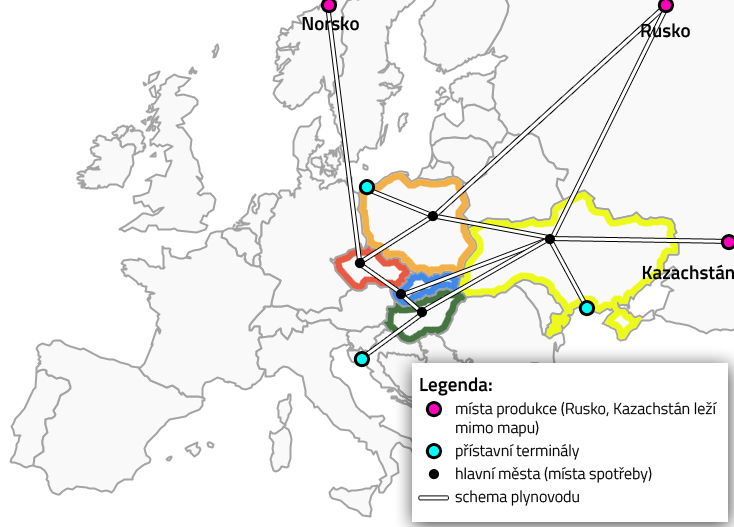
\includegraphics{Geo-map-europe-contour-map.jpg}}
\end{center}
\caption{Abstraktní schéme systému.}
\label{evropa}
\end{figure}

V modelu dochází k zahájení zásobování jednotlivých zemí až po určité době běhu
programu\footnote{Doba přepravy mezi místem produkce a jednotlivou zemí}.
Důvodem je zpoždění vyvolané prvnotní přepravou plynu z místa produkce do místa spotřeby.
Tento fakt může být zanedbán, jelikož neovlivní výsledky navržených
scénářů\footnote{Pokud by byla potřeba tuto skutečnost nezanedbávat,
docílilo by se toho například zvýšením počátečních zásob zemí o hodnotu,
která se spotřebuje, než dojde první dodávka plynu.}.

\section{Architektura simulačního modelu/simulátoru}

%Tato kapitola má různou důležitost pro různé typy zadání. U implementačních témat lze tady očekávat jádro dokumentace. Zde můžete využít zajímavého prvku ve vašem simulačním modelu a tady ho "prodat".
%kapitola 4.1: Minimálně je nutno ukázat mapování abstraktního (koncept.) modelu do simulačního (resp. simulátoru). Např. které třídy odpovídají kterým procesům/veličinám a podobně.

Vzhledem k jednoduchosti modelu a použití
disktrétního času \cite[str,22]{IMS} byla vybrána koncepce,
kdy jádro programu tvoří cyklus \texttt{while}, ve kterém se
vykonávají akce transportu, spotřeby, exportu a importu.
Odlišnost v jednotlivých typech simulací je ve funkcích
použitých pro inicializaci struktur, které reprezentují
jednotlivé prvky modelovaného systému.

\subsection{Struktury a inicializace}

Jednotlivé struktury se liší svými parametry.
Například struktura reprezentující terminál obsahuje položky pro reprezentaci cílového uzlu v síti,
množství přenášeného plynu a dobu přenosu.
Oproti tomu struktura reprezentující transport obsahuje navíc ještě položku reprezentující zdroj.
Struktura určená pro reprezentaci států (míst spotřeby), pak obsahuje položky pro maximální velikost zásobníku,
aktuální stav plny, spotřebu a  produkci.

\subsection{Vektor transakcí}

Vzhledem k tomu, že není využito simlačních knihoven, dochází k absenci kalendáře událostí.
Přestože jsou zpracovávány události po každé hodině modelového času,
bylo nutné implementovat způsob zpracování událostí v určitém čase.
Pro tyto účely byl vytvořen \textbf{vektor transkací}, do něhož jsou ukládány události,
které se mají vykonat až po určitém čase.
Tyto události se týkají přenosu, spotřeby a produkce zemního plynu.
Nejprve je potřeba plyn odečíst ze zásob odesílající země a až po nějakém čase mají být uloženy do zásobníku v cílové zemi.

Obsah vektoru tvoří struktury s položkami reprezentujícími cílovou zemi,
čas přenosu a množství zemího plynu, které je přenášeno.
Tento vektor je po každé hodině modelového času procházen a časy u jednotlivých záznamů jsou dekrementovány.
Pokud čas dosáhne hodnoty 0, je tato transakce dokončena\footnote{Plyn je uložen v zásobníku cílové stanice a záznam je z vektoru transakcí odstraněn}. 

\subsection{Zpracování akcí}

Zpracování akcí se dá rozčlenit do několika částí, které se opakují.
Nejprve se vloží informace o importu plynu od přístavních terminálů do vektoru transakcí,
poté se spotřebuje plyn a exportuje se do zemí mimo modelovaný systém.
Následovně se vloží do vektoru transakcí informace o přesunu plynu mezi jednotlivými zeměmi
a odečte se dané množství od zásob zdrojové země.

Na závěr se provede průchod vektorem transakcí a transakce,
jež mají být provedeny v aktuálním čase se provedou\footnote{funkce \texttt{transakceCheck()}}. 

\subsection{Modelový čas}

Modelový čas byl zvolen jedna hodina a tato jedna hodina odpovídá jedné iteraci hlavního cyklu while.

Aby model odpovídal reálnému světu, bylo do něj potřeba zanést střídání letního a zimního období
\footnote{letní období duben až září, zimní období říjen až březen}.
Důvodem tohoto požadavku byla značná rozdílnost ve spotřebě zemního plynu jednotlivých míst spotřeby
v různých obdobích (v letním období menší spotřeba, v zimním větší).
Změny období bylo docíleno pomocí počítadla cyklů, jehož hodnota se v každé iteraci porovnává 
s aktuální hodnotou značící začátek nového období, pokud jsou hodnoty totožné 
je hodnota značící začátek nového období navýšena o hodnotu 182\footnote{hodnota 182 značí půlku jednoho roku}
a spotřeba jednotlivých států je přepnuta na hodnotu odpovídající danému období.

Inicializační hodnota hodnoty značící začátek nového období je 90 \footnote{90 den odpovídá počátku dubna - počátku letního období}
a tímto je docíleno, že modelový čas odpovídá svým začátkem pomyslnému začátku roku reálného světa.

\section{Podstata simulačních experimentů a jejich průběh}

Nezaměňujte pojmy testování a experimentování (důvod pro bodovou ztrátu)!!!
Zopakovat/shrnout co přesně chcete zjistit experimentováním a proč k tomu potřebujete model. Pokud experimentování nemá cíl, je celý projekt špatně. Je celkem přípustné u experimentu odhalit chybu v modelu, kterou na základě experimentu opravíte. Pokud se v některém experimentu nechová model podle očekávání, je nutné tento experiment důkladně prověřit a chování modelu zdůvodnit (je to součást simulačnické profese). Pokud model pro některé vstupy nemá důvěryhodné výsledky, je nutné to zdokumentovat. Pochopitelně model musí mít důvěryhodné výsledky pro většinu myslitelných vstupů.
\subsection{Postup experimentování}

kapitola 5.1: Naznačit postup experimentování – jakým způsobem hodláte prostřednictvím experimentů dojít ke svému cíli (v některých situacích je přípustné "to zkoušet tak dlouho až to vyjde", ale i ty musí mít nějaký organizovaný postup).
\subsection{Jednotlivé experimenty}
kapitola 5.2: Dokumentace jednotlivých experimentů - souhrn vstupních podmínek a podmínek běhu simulace, komentovaný výpis výsledků, závěr experimentu a plán pro další experiment (např. v experimentu 341. jsem nastavil vstup x na hodnotu X, která je typická pro ... a vstup y na Y, protože chci zjistit chování systému v prostředi ... Po skončení běhu simulace byly získány tyto výsledky ..., kde je nejzajímavější hodnota sledovaných veličin a,b,c které se chovaly podle předpokladu a veličin d,e,f které ne. Lze z toho usoudit, že v modelu není správně implementováno chování v podmínkách ... a proto v následujících experimentech budu vycházet z modifikovaného modelu verze ... Nebo výsledky ukazují, že systém v těchto podmínkách vykazuje značnou citlivost na parametr x ... a proto bude dobré v dalších experimentech přesně prověřit chování systému na parametr x v intervalu hodnot ... až ...)
kapitola 5.3: Závěry experimentů – bylo provedeno N experimentů v těchto situacích ... V průběhu experimentování byla odstraněna ... chyba v modelu. Z experimentů lze odvodit chování systémů s dostatečnou věrohodností a experimentální prověřování těchto ... situací již napřinese další výsledky, neboť ...


\section{Shrnutí simulačních experimentů a závěr}

Závěrem dokumentace se rozumí zhodnocení simulační studie a zhodnocení experimentů (např. Z výsledků experimentů vyplývá, že ... při předpokladu, že ... Validita modelu byla ověřena ... V rámci projektu vznikl nástroj ..., který vychází z ... a byl implementován v ...).
do závěru se nehodí psát poznámky osobního charakteru (např. práce na projektu mě bavila/nebavila, ...). Technická zpráva není osobní příběh autora.
absolutně nikoho nezajímá, kolik úsilí jste projektu věnovali, důležitá je pouze kvalita zpracování simulátoru/modelu a obsažnost simulační studie (rozhodně ne např.: projekt jsem dělal ... hodin, což je víc než zadání předpokládalo. Program má ... řádků kódu). Pokud zdůrazňujete, že jste práci dělali významně déle než se čekalo, pak tím pouze demonstrujete vlastní neschopnost (to platí zejména v profesním životě).
do závěru se velmi nehodí psát "auto-zhodnocení" kvality práce, to je výhradně na recenzentovi/hodnotiteli (např. v projektu jsem zcela splnil zadání a domnívám se, že můj model je bezchybný a výsledky taktéž). Statisticky častý je pravý opak autorova auto-zhodnocení. Pokud přesto chcete vyzdvihnout kvalitu svého díla (což je dobře), tak vaše výroky musí být naprosto nepopiratelně zdůvodněny a prokázány (např. pomocí jiného referenčního přístupu, matematického důkazu, analýzy, ...).


\newpage
\renewcommand{\refname}{Literatura a použité zdroje}
\begin{thebibliography}{99}
\bibitem{IMS}P. Peringer: přednášky předmětu Modelování a simulace
https://www.fit.vutbr.cz/study/courses/IMS/public/prednasky/IMS.pdf	
\bibitem{IEA} IEA natural gas information [online]. [cit. 2014-12-03]. ISBN 1683-4267. Dostupné z: http://www.oecd-ilibrary.org/energy/natural-gas-information{\_}16834267
\bibitem{GIE} Gas Infrastructure Europe [online]. [cit. 2014-12-03]. Dostupné z: http://www.gie.eu.com/
\bibitem{Mapka staty} http://www.gie.eu.com/download/maps/ENTSOG-GIE{\_}SYSDEV{\_}MAP2013.pdf
\bibitem{engineering} Natural gas engineering and safety challenges. pages cm. ISBN 978-331-9089-478.
\bibitem{lngeurope}Gas LNG Europe. [online]. [cit. 2014-12-07].Dostupné z:http://www.gie.eu/down-
load/maps/2014/GLE{\_}LNG{\_}JUNE2014.pdf
\bibitem{lngkrk}O PROJEKTU. ADRIA LNG [online]. [cit. 2014-12-07]. Dostupné z: http://www.adria-lng.hr/index.php?f={\&}m=2{\&}s=0
\bibitem{lngukrajina}Ukraine LNG Terminal, Ukraine. [online]. [cit. 2014-12-07]. Dostupné z: http://www.hydrocarbons-technology.com/projects/ukraine-lng-terminal/
\end{thebibliography}
\end{document}
